% TODO: Convert code over to Psi4 so all work can be done inside Jupyter notebooks
% Tutorial prepared by Igor Y. Zhang, Hagen-Henrik Kowalski and Tonghao Shen 2017.
% Transcribed and modified by Dustin D. Wheeler
% Updated 2021
\documentclass[nobib,nofonts,nols,nohyper]{tufte-handout}
%% Header file cloned from https://github.com/wickles/latex-base

%%%%%%%%%%%%%%%%%%
%% CONTENTS
%%%%%%%%%%%%%%%%%%
% To-do / issues
% Packages
% Commands
% Special Symbols
% Environments
% More commands: Resizable delimiters
% More commands: Derivatives
% Useful templates
% Notes
%%%%%%%%%%%%%%%%%%
%%%%%%%%%%%%%%%%%%



%%%%%%%%%%%%%%%%%%
%% TO-DO / ISSUES
%%%%%%%%%%%%%%%%%%

%% packages
% Replace physics package with alternatives
% - Physics replacements
% 	- braket
% 	- derivative (need tectonic to support TeXLive 2021)
% 	- vectors?
% Update commands for siunitx (requires TeXLive 2021)




%%%%%%%%%%%%%%%%%%
%% PACKAGES
%%%%%%%%%%%%%%%%%%


%% debugging / diagnostics
\RequirePackage[l2tabu,orthodox]{nag} % nags user about obsolete and improper syntax

\usepackage{xparse} % provides high-level interface for producing document-level commands
	% via \[Declare/New/Renew/Provide/etc]DocumentCommand
	% allows for more than one optional argument in commands

\usepackage{iftex,ifluatex,ifxetex,ifdraft} % check if a document is being processed with pdfTeX, or XeTEX, or LuaTEX
\newif\ifxetexorluatex % a new conditional starts as false, true if using XeTeX OR LuaTeX
\ifnum 0\ifxetex 1\fi\ifluatex 1\fi>0
   \xetexorluatextrue
\fi

%% fonts and encoding 

% standard and structural packages

% \newcommand\bmmax{4} % increase max number of bm font allocations. default 4?
% \newcommand\hmmax{1} % increase max number of hm font allocations. default 3?
\usepackage{bm} % provides \bm command for robustly bolding math characters

%%%%%%%%%%%%%%%%%%%%%% Additional math fonts %%%%%%%%%%%%%%%%%%%%%%%%%%%%%%%%%%%
\usepackage{amssymb} % for \mathbb (upper case only), \mathfrak fonts
%%%%%%%%%%%%%%%%%%%%%%%%%%%%%%%%%%%%%%%%%%%%%%%%%%%%%%%%%%%%%%%%%%%%%%%%%%%%%%%%%

\usepackage{microtype} % improves kerning in certain cases. 
	% recommended to disable protrusion in table of contents!

%% Latex interface 

\usepackage{letltxmacro} % provides \LetLtxMacro command for correct renaming of commands
\usepackage{etoolbox} % provides many useful programming tools, 
	% e.g. \ifdefempty{cs}{true}{false}



%% media interface

\usepackage{graphicx} % support the \includegraphics command and options
\usepackage{subfig} % Support for subfigures and subcaptions
	\captionsetup[subfloat]{position=bottom}
% \makeatletter%
% \@ifclassloaded{tufte-handout}% xcolor is pre-loaded with the tufte-latex package
%   {
	% \ifxetexorluatex % if lua- or xelatex http://tex.stackexchange.com/a/140164/1913
		\newcommand{\textools}[2][5]{%
			\begingroup\addfontfeatures{LetterSpace=#1}#2\endgroup
		}
		\renewcommand{\allcapsspacing}[1]{\textools[15]{#1}}
		\renewcommand{\smallcapsspacing}[1]{\textools[10]{#1}}
		\renewcommand{\allcaps}[1]{\textools[15]{\MakeTextUppercase{#1}}}
		\renewcommand{\smallcaps}[1]{\smallcapsspacing{\scshape\MakeTextLowercase{#1}}}
		\renewcommand{\textsc}[1]{\smallcapsspacing{\textsmallcaps{#1}}}
% 	\else
% 	\fi
% }%
%   {\usepackage[dvipsnames,svgnames,table,hyperref]{xcolor}
% 	% provides access to large number of colors and related features
% 	% see end notes for lists of available colors
% 	}%
% \makeatother%
\usepackage{svg} % provides \includesvg command for svg figures. 
\usepackage{pgfplots} % for plotting in tikzpicture environment
	\pgfplotsset{compat=1.16} % required to select newest version
\usepackage{tikzscale} % allows \includegraphics{*.tikz} and scaling of TiKZ images


%% math interface

\usepackage{amsmath} % for nice math commands and environments
\usepackage{mathtools} % extends amsmath with bug fixes and useful commands, e.g.
	% \shortintertext for short interjections in align environment,
	% \prescript{t}{b}{X} for simple, nicely aligned math pre-(super/sub)scripts
	% \Aboxed{...} for boxing full lines in 'align' environment
\usepackage{array} % improves array support, esp. in tabular env. 
	% see also xtab.sty
\usepackage{booktabs} % allows for improved spacing in tabular env. 
	% use \toprule, \*midrule, \bottomrule instead of \hline
	% see also ctable.sty

\usepackage{derivative} % provides \odv, \pdv, \odif, \pdif
\usepackage{bropd} % provides \br command which simplifies nesting of bracketed terms 
	% e.g. \br{\br{x-a}^2+\br{y-b}^2} produces \left[ \left( x-a \right)^2 + \left( y-b \right)^2 \right]


%% Science and programming packages
\usepackage{fvextra} % for verbatim and comment environments with \Verb
\usepackage{chemmacros} % for writing chemical formulas with \ch, e.g. \ch{AgCl2-} or \ch{^{227}_{90}Th+}
	\usechemmodule{
		spectroscopy, % provides 
    thermodynamics, % provides state variables and equations
    units, % provides \[mM]olar, \Torr, \atm, \cal, \cmc, \MolMass
		} % also loads siunitx and chemformula
	\DeclareSIUnit\ppm{ppm}
  \sisetup{% siunit package options
			per-mode = symbol,%
			inter-unit-product=\ensuremath{{}\!\cdot\!{}},%
			separate-uncertainty,%
			multi-part-units = single,%
			retain-explicit-plus,%
			list-final-separator={, and },%
			math-celsius = °\text{C}, % for temperatures
			text-celsius = °C,
			math-degree = °, % for angles
			text-degree = °}%


\usepackage{physics} % provides streamlined interface with many commands to simplify
	% writing standard physics notation (bra-kets, derivatives, etc.)
	% differentials and derivatives: \dd[n]{x}, \dv[n]{f}{x}, \dv{x}, \pdv{f}{x}{y}, \var{Q}, \fdv{F}{g}
	% bra-ket notation: \bra, \ket, \braket, \dyad, \matrixel 
	% \qty(x) for delimited quantities
	% \abs, \norm, \eval, \order ,\comm, \acomm
	% vectors: \vb, \va, vu, \vdot, \cross, \grad, \div, \curl, \laplacian
	% largely replaces and adds basic math functions with auto-delimiters: trig, linear algebra, etc.
		% no inverse hyperbolic trig? 
	% in particular adds \tr, \Tr, \rank, \erf, \Res, \pv / \PV, \Re, \Im
	% auto padding text: \qq{string}
	% matrix quantities: \mqty(a & b \\ c & d) or \mqty[x \\ y], Pauli \pmat{n}, diagonal matrices \mqty(\dmat{1,2&3\\4&5}), anti-diagonal \admat

%% misc packages

\usepackage{datetime} % allows easy formatting of dates, e.g. \formatdate{dd}{mm}{yyyy}
%\usepackage[inline]{enumitem} % allows for custom labels on enumerated lists
	% e.g. \begin{enumerate}[label=\textbf{(\alph*)}]
	% label options are: \alph, \Alph, \arabic, \roman, and \Roman
	% inline option creates '*' versions of enumerate, itemize, description 
		% which can be inlined within the text of a paragraph. 
% \usepackage{outlines} % provides 'outline[style]' environment, allowing for subitems in lists
	% e.g. \begin{outline} \1 item \2 subitem \3[A)] subsubitem \1 item \end{outline}
	% or with other style: \begin{outline}[enumerate], etc

% \usepackage{rotating}
	% provides environments for rotating arbitrary objects, e.g. sideways, turn[ang], rotate[ang]
	% also provides macro \turnbox{ang}{stuff}
%\usepackage{ctable} % allows for footnotes under table and properly spaced caption above 
	% must be loaded after tikz
	% incorporates (..?)
\usepackage{framed} % provides boxed 'framed' environment for easily boxing text 
\usepackage{tcolorbox}
	\tcbuselibrary{skins, breakable, xparse, minted}
	% provides fancier boxes than regular \makebox, \fbox, etc.
	% e.g. \doublebox, \ovalbox, \shadowbox
	% Can use `\tcbuselibrary{listings}` to use the listings library, 
		% doesn't require a language to be defined. 
\usepackage{empheq} % provides 'empheq' environment 
	% for improved control over shape, size, color of framed boxes, e.g. 
\newcommand{\boxedeq}[2]{
	\begin{empheq}[box={\fboxsep=6pt\fbox}]{align}\label{#1}#2\end{empheq}
}
\newcommand{\coloredeq}[2]{
	\begin{empheq}[box=\colorbox{lightgreen}]{align}\label{#1}#2\end{empheq}
}


%% document interface 

\usepackage{footnote} % 
\usepackage{hyperref} % adds hyperlinks and outline to PDF documents
	\hypersetup{%
		pdfencoding=auto,%
		psdextra,%
		pdfusetitle,%
		colorlinks=true,%
		linkcolor=BrickRed, %
		citecolor=Green, %
		filecolor=Mulberry, %
		urlcolor=NavyBlue, %
		menucolor=BrickRed, %
		runcolor=Mulberry, %
		linkbordercolor=BrickRed, %
		citebordercolor=Green, %
		filebordercolor=Mulberry, %
		urlbordercolor=NavyBlue, %
		menubordercolor=BrickRed, %
		runbordercolor=Mulberry %
		} %
	% options enable enhanced unicode and math support in PDF outlines [causes conflict with \C command?]
\usepackage{cleveref} % provides \cref command which inserts contextually correct word in front of ref.
	% e.g. \cref{eq:myeq} --> Equation 1.2, or so
\usepackage{bookmark} % improves package hyperref's bookmarking. 
	% properties such as style and color can be set. Generates bookmarks in first run. 

%% font packages -- load fontenc, then inputenc, then lmodern. 
% see http://tex.stackexchange.com/a/44699
\usepackage{fontspec}
\usepackage[math-style=ISO]{unicode-math} 
\ifdraft{}{
	\setmainfont{STIX2Text}[
		Extension={.otf},
		UprightFont={*-Regular},
		BoldFont={*-Bold},
		ItalicFont={*-Italic},
		BoldItalicFont={*-BoldItalic},]
	\setmathfont{STIX2Math}[
		Extension={.otf}]
}
	\renewcommand{\vb}[1]{\symbf{#1}} % fix vector command from physics package to work with unicode-math


%% load later packages
\usepackage{lineno} % provides line numbers in main text for reference and peer review
	% activated by calling \linenumbers in document
\usepackage[textsize=footnotesize]{todonotes}





%%%%%%%%%%%%%%%%%%
%% COMMANDS
%%%%%%%%%%%%%%%%%%

% \newcommand{\mtext}[1]{{\textnormal{#1}}} % for writing text within math mode, e.g. for subscripts
\LetLtxMacro{\mtext}{\text} % legacy alias for \mtext
% \LetLtxMacro{\opname}{\operatorname} % custom operator names
% %\newcommand{\tr}{\opname{tr}} % for trace
% %\newcommand{\rank}{\opname{rank}} % for rank
% \newcommand{\diag}{\opname{diag}} % i.e. \diag(\lambda_1, \dots, \lambda_n)
% \LetLtxMacro{\fancyRe}{\real} % already renamed from physics.sty
% \LetLtxMacro{\fancyIm}{\imaginary} % see above
% \renewcommand{\Re}{\opname{Re}}
% \renewcommand{\Im}{\opname{Im}}
% \renewcommand{\Res}{\opname*{Res}} % for residue function (handles limits properly)
% \newcommand{\inv}{^{-1}}
% \newcommand{\sgn}{\opname{sgn}} % sign/signum function
\DeclareMathOperator{\sgn}{sgn}
\DeclareMathOperator{\erfc}{erfc}
\DeclareMathOperator{\GammaFunc}{\symup{\Gamma}}
\newcommand{\iu}{\TextOrMath{$\mtext{i}$}{\mtext{i}\mkern1mu}}
%
% \newcommand{\laplacian}{\nabla^2}

%% pre-defined colors
% standard: black, blue, brown, cyan, darkgray, gray, green, lightgray, lime, magenta, olive, orange, pink, purple, red, teal, violet, white, yellow
%
% dvips: Apricot, Aquamarine, Bittersweet, Black, Blue, BlueGreen, BlueViolet, BrickRed, Brown, BurntOrange, CadetBlue, CarnationPink, Cerulean, CornflowerBlue, Cyan, Dandelion, DarkOrchid, Emerald, ForestGreen, Fuchsia, Goldenrod, Gray, Green, GreenYellow, JungleGreen, Lavender, LimeGreen, Magenta, Mahogany, Maroon, Melon, MidnightBlue, Mulberry, NavyBlue, OliveGreen, Orange, OrangeRed, Orchid, Peach, Periwinkle, PineGreen, Plum, ProcessBlue, Purple, RawSienna, Red, RedOrange, RedViolet, Rhodamine, RoyalBlue, RoyalPurple, RubineRed, Salmon, SeaGreen, Sepia, SkyBlue, SpringGreen, Tan, TealBlue, Thistle, Turquoise, Violet, VioletRed, White, WildStrawberry, Yellow, YellowGreen, YellowOrange

\usepackage[mackeys=text]{menukeys}
  \usetikzlibrary{arrows.meta}
  \tikzset{menukeys key symbol/.style={>=Triangle}} % Change Arrow headers for key symbols
  \DeclareSIUnit\kcal{kcal}
  \DeclareSIUnit\wn{\raiseto{-1}\cm}
  \DeclareSIUnit\hartree{Ha}

%%%%%%% Bibliography options %%%%%%%%%%%%%%%%%%%%%%%%%%%%%%%%%%%%%%%%%%%%%%%%%
% (fold)
\usepackage[%
  style=numeric-comp,%
  sortcites,%
  sorting=none,%
  defernumbers=true,%
  hyperref,
  backend=biber,
  ]{biblatex}
  \addbibresource{../../pchem_bib.bib}

  % Filter bibliography file to only include entries matching keyword.
  \DeclareSourcemap{%
    \maps[datatype=bibtex]{%
      \map{%
        \step[nocited, final]%
        \step[fieldsource=keywords, notmatch=compchem, final]%
        \step[entrynull]%
      }%
    }%
  }

  % Add a section for cited bibliography entries.
  % At the end, create a second bibliography for uncited items (Further Reading).
  \DeclareBibliographyCategory{cited}
  \AtEveryCitekey{\addtocategory{cited}{\thefield{entrykey}}}

  % Define a style for the Further Reading section
  \defbibenvironment{nolabelbib}
    {\list
       {}
       {\setlength{\leftmargin}{2\bibhang}%
        \setlength{\itemindent}{-\bibhang}%
        \setlength{\itemsep}{\bibitemsep}%
        \setlength{\parsep}{\bibparsep}}}
    {\endlist}
    {\item}

  % Remove URL from citations if DOI is present.
  \AtEveryBibitem{%
    \iffieldundef{doi}{ % do nothing if true
    }
    { % otherwise, clear the URL
      \clearfield{url}
    }%
  }
% (end)

%%%%%%% Source Code options %%%%%%%%%%%%%%%%%%%%%%%%%%%%%%%%%%%%%%%%%%%%%%%%%%

% Command to insert $PROMPT before shell console input
\newcommand{\BashFancyFormatLine}{%
  \def\FancyVerbFormatLine##1{\textcolor{blue}{\small user:\char`\~\$}\ ##1}%
}

% Set up Gaussian input settings
\tcbuselibrary{listings} % Use listings library for dummy Gaussian input files.
	\lstset{morecomment=[s]{<}{>}} % Set comment style for dummy Gaussian input

% tcolorbox settings for code blocks
\tcbset{
  colback=blue!4!white,
  colframe=blue!85!black,
  listing only,
  left=1.5em,
  enhanced jigsaw,
  breakable,
  overlay={
    \begin{tcbclipinterior}
      \fill[red!20!blue!20!white] 
      (frame.south west)  rectangle 
      ([xshift=1.5em]frame.north west);
    \end{tcbclipinterior}}
}
\setminted{
  style=tango,
  fontsize=\small,
  breaklines,
  breakafter=|,
  autogobble,
  linenos,
  numberfirstline=true,
  firstnumber=1,
  stepnumber=2,
  numbersep=1em
}

% Settings for all code blocks
\lstset{
  breaklines=true,
  basicstyle=\small,
  numberstyle=\tiny,
  numbers=left,
  numberfirstline=true,
  firstnumber=1,
  stepnumber=2,
  numbersep=2em,
}

% Settings for Gaussian code blocks
\lstdefinestyle{gaussian}{
  language=Clean,
  % keywordstyle=\bfseries,
  commentstyle=\slshape,
  % stringstyle=\ttfamily,
  numbers=left,
  firstnumber=1,
  stepnumber=2,
  numberfirstline=true,
  numbersep=2em,
  numberstyle=\tiny,
  breaklines=true,
  breakautoindent=true,
  tabsize=2,
  basicstyle=\ttfamily\small,
  showspaces=false,
  showstringspaces=false,
  morecomment=[s]{<}{>}
}

% Minted settings for inline bash code
\newmintinline{bash}{}

% Hack to force linebreaks at `¬` in bashinputs. From
% https://tex.stackexchange.com/a/461455/27032
\AtBeginEnvironment{bashinput}{%
  \catcode`¬\active
  \begingroup\lccode`~=`\¬\lowercase{\endgroup\def~{\linebreak}}%
}

% Settings for bash code blocks
\newtcblisting{bashinput}[1][]{
  listing engine=minted,
  minted language=bash, 
  listing only,
  minted options={,
    formatcom=\BashFancyFormatLine
  },
  #1
}

% Settings for Gaussian input file blocks
\newtcblisting{gaussinput}[1][]{
	listing engine=listings,
	listing only,
  listing options={
    style=gaussian
    },
  #1
}
%%%%%%%%%%%%%%%%%%%%%%%%%%%%%%%%%%%%%%%%%%%%%%%%%%%%%%%%%%%%%%%%%%%%%%%%%%%%%%%

\begin{document}

\title{Introduction to Computational Chemistry}

\author{Dustin Wheeler, Mateusz Marianski}

\begin{document}

\maketitle

\begin{abstract}
  This tutorial aims to give a basic introduction to electronic structure calculations for very simple systems.\thanks{Adapted from \textcite{marianski19}.} 
  As every quantum chemistry code has its own philosophy, this tutorial should familiarize you with the general-purpose Gaussian16 (hereafter abbreviated as g16) software.
  The experiments will also demonstrate the predictive power of quantum-chemical calculations. 	
	
  First, the basic structure of an input file to the G16 software will be explained.
  The second part will introduce scanning along the binding curve and computing observables. 
  The third part introduces geometric optimization of a small molecule and how to assess reliability of the result. 

  \begin{enumerate}[
      label=Prob. \Roman*:,
      align=left,
      leftmargin=*,
      itemindent=\parsep
    ]
    \item \hyperref[sec:problemI]{The hydrogen atom}
    \item \hyperref[sec:problemII]{Hydrofluoric acid: bond length and dipole moment}	      
    \item \hyperref[sec:problemIII]{Hydronium cation: geometry relaxation, vibrations, and PES}
  \end{enumerate}

As the first step, please use this link to clone the files into your Jupyter directory:\\  \href{https://sugarcube.hunter.cuny.edu/hub/user-redirect/git-pull?repo=https%3A%2F%2Fgithub.com%2Fmskblackbelt%2Fpchem_comp-chem_template&urlpath=lab%2Ftree%2Fpchem_comp-chem_template%2FCompChem_template.ipynb&branch=main}{\texttt{https://tinyurl.com/chem357-compchem}}
\marginnote[-4\baselineskip]{While working through this lab, do \textbf{not} copy and paste the code in this PDF into your input files. Invisible formatting characters are often copied from the PDF. Gaussian will not understand these characters and your calculations will not start.}

This guide is meant to be used in tandem with the Jupyter notebook contained in the cloned folder (``pchem\_comp-chem\_template/CompChem\_template.ipynb''). 
That notebook has a number of cells pre-populated for your convenience. Make sure you read the notes and comments in the notebook as you go through the lab and fill in any blanks before executing the cells. 
\end{abstract}



%!TEX root = ./Intro_to_CC.tex

\section{A first look at the Shell and Gaussian16}

The work in this lab will take place partly in a Jupyter notebook and partly in the Terminal program. You can open Terminal from the JupyterLab launcher or from the menu under \menu{File>New}. 
Prior to beginning work, you should familiarize yourself with the Bash shell by running through the exercises from DigitalOcean available at \url{https://www.digitalocean.com/community/tutorial_series/getting-started-with-linux} (except the part on Linux Permissions, as it isn't relevant). 

The most common Bash commands are available for your reference in the appendix. 
Before starting, make sure you understand how to navigate the file system with \Verb{pwd}, \Verb{ls}, and \Verb{cd}, and that you can copy, move, and remove a sample file using the \Verb{cp}, \Verb{mv}, and \Verb{rm} commands. 
Also make sure you understand the difference between \emph{relative} and \emph{absolute} file paths.\sidenote{Hint: read the appendix!}

It is a good practice to perform each calculation a separate directory. The calculations are initialized by calling the \Verb{g16} command on an input file:\sidenote{This input represents commands typed into the shell. The leading characters in blue (everything up to the dollar sign) represent the user prompt and should not be typed.}
\begin{bashinput}
  g16 input &
\end{bashinput}
	
By convention, the input file is named \Verb{input.com}, though any name will work. 
The basic input file is shown below.\sidenote{Content wrapped in angle brackets (\Verb{<*>}) should be \textbf{replaced} with the desired value and the angle brackets should be \textbf{removed} (they are not a recognized Gaussian input), e.g., \Verb{<basis>} \( \Rightarrow \) \Verb{STO-3G}.}
This file starts a calculation on two processors using \qty{400}{\mega\byte} of memory. 
The output will be redirected to the \Verb{input.log} output file. 
This file contains the basic information and results of the calculation such as the total energy, atomic forces, and so forth. 
Additional output files might be generated according to the specified settings. 
Individual components of the input file are described below. 
\begin{gaussinput}[title=Structure of a simple input file, 
label=lst:gauss_samp]
%nproc=2
%mem=400MB
#<method> <basis-set>
#sp scf=tight
    <empty line>
<title information>
    <empty line>
<charge> <multiplicity>
<atom1>   <x1>	<y1>	<z1>
<atom2>   <x2>	<y2>	<z2>
 ... 
<atomN>   <xN>	<yN>	<zN>
    <empty line>
\end{gaussinput}

\begin{description}[font=\ttfamily\upshape]
  \item[\%nproc=2] This keyword specifies the number of processors that will be employed for calculations. The computer you are using has 2 processing cores and you should use them all. 
  \item[\%mem=400MB] This keyword manages the maximum memory usage during the calculations. The most efficient memory specification is beyond this tutorial. 
  \item[method] Substitute \Verb{<method>} with the method of choice for electron--electron interactions. In this tutorial, we will use several methods, namely Hartree-Fock (HF), Møller-Plesset second order perturbation theory  (MP2) and a few density-functionals. The details of each method will be covered in detail during the lecture. 
  \item[basis-set] Substitute the \Verb{<basis-set>} word with the desired basis set. This specifies a set of basis functions (for instance atomic orbitals, gaussian-type orbitals, plane waves) that will be used to express an electronic configuration. The recommended basis sets are specified in each exercise. 
  \item[sp] The \Verb{sp} command orders Gaussian to perform single-point calculations, i.e., energy evaluation of a specified structure using \Verb{method} and \Verb{basis-set}
  \item[scf=tight] The Schrödinger equation is solved in self-consistent manner. The \Verb{scf=tight} option specifies tight convergence criteria for the self-consistent cycle. 
  \item[your-comment] This line, surrounded by two empty lines, holds your comment, usually a description of the molecule and/or calculation to be performed. 
  \item[charge] The \Verb{charge} keyword should be substituted with the total (integer-valued) charge of your system. 
  \item[multiplicity] The \Verb{multiplicity} keyword should be substituted with the multiplicity of your system (\( 2\mtext{S}+1 \), where \( \mtext{S} \) is total spin). This should always be an integer.
  \item[atomX <X> <Y> <Z>] This block specifies the geometry of the system. You can use either the atomic symbol (e.g., \Verb{C}) or the atomic number (e.g., \Verb{6}) to specify the atom type, followed by it's cartesian coordinates in units of Angstroms (\unit{\angstrom}).\sidenote{Use a decimal-valued coordinate, even if it is a whole number (\Verb{0.0}, not \Verb{0}).} This block must be followed by an empty line. 
\end{description}

Remember, there are no bonds (sticks) in quantum chemistry. The bonding is the result of the respective positions of atoms in space. The `stick' visible in visualization programs is simply a rendering for more intuitive display. A sample input for a square-planar molecule can be found at the end of the section (with all values filled in). 


\subsection{Additional tools and programs}

\begin{description}[font=\bfseries]
  \item[Bash shell] A short list of the basic bash (command line) commands is given in the appendix. 
  \item[Text editor] JupyterLab comes with a built-in text editor. Most files can be opened and edited by double-clicking their icon in the file browser panel on the left side of the window. Occasionally, you will run into files with an extension that opens a different program (e.g., CSV files open the CSV viewer, which can't edit by default). In these cases, you'll have to click ``File > Open from Path…'' and give the full path to the file. 
  New files can be created by clicking ``File > New > Text File'' or clicking on the Text File icon in the launcher. 
  Another option is the command line text editor \Verb{vim}. 
  When working from the command line, this program is (almost) always available.
  If you plan on continuing with computer work, it would behoove you to learn the basics of Vim.  
  A number of introductions to Vim are available online. Two such examples are \url{https://www.openvim.com} and \url{https://vim-adventures.com/}.
  \item[Scripts] For some exercises, scripts are required for dedicated tasks. All scripts you will need for this tutorial can be found in their respective directories. 
\end{description}

\begin{gaussinput}[title=A sample \Verb{input.com} file for the \ch{XeF4} molecule.]
%nproc=2
%mem=400MB
# b3lyp 6-31g
# sp scf=tight

Xenon tetrafluoride single point DFT calculation

0 1
Xe  0.0   0.0   0.0
F   1.0   0.0   0.0
F   0.0   1.0   0.0
F  -1.0   0.0   0.0
F   0.0  -1.0   0.0

\end{gaussinput}
%!TEX root = ./Intro_to_CC.tex

\section{Problem 1: The hydrogen atom} % (fold)
\label{sec:problemI}

In this exercise, we will look at different basis sets using the hydrogen atom. The hydrogen atom is the only non-trivial system for which the exact analytic solution is known. 
By the end of the first exercise, we will see how various computational methods compare to each other and to the exact solution.  
From a technical perspective, we will learn how to compose input files, run basic Gaussian calculations, search for energy in the Gaussian output, and perform basis set convergence tests.

\subsection*{Getting started - the hydrogen atom}
%\task{
%\textbf{Tasks:}
%  \begin{itemize}
%  \item Generate a simple \geometryin{} and \controlin{} file and run FHI-aims.
%  \item Test the convergence of the total energy with basis size.
%  \item Compare the total energy of the hydrogen atom computed with different methods implemented in FHI-aims. Do all methods converge to the same result?
%  \end{itemize}%
%}
%
%\noindent
%\task{
%\textbf{Educational Objectives:}
  %\begin{itemize}
  %\item Become aquainted with running FHI-aims calculations
  %\item Generate a \controlin and \geometryin file.
  %\item Learn how to do systematic basis set convergence
  %\end{itemize}
%}



\textbf{Tasks}
\begin{enumerate}
  \item First, go to the \Verb{Problem_1} directory by typing in the terminal \bashinline{cd ~/pchem_comp-chem_template/Problem_1}. 
  There, create a test directory (\bashinline{mkdir "name_of_directory"}) with a name of your choosing. 
  Inside it, generate a simple \Verb{input.com} file (\menu{File>New>Text File}) which contains only a single hydrogen atom, using the example shown in the introduction. 
  This corresponds to a single hydrogen atom in a hypothetical ideal gas phase. 
  It is located at the origin of the coordinate system, although its position does not matter here.
 
  \item For the method, use \Verb{HF} (Hartree-Fock method) and minimal \Verb{STO-3G} basis set which represents each available atomic orbital with three contracted gaussian functions.\sidenote{Gaussian commands are not case-sensitive, so \texttt{HF} is the same as \texttt{hf}, \texttt{Hf}, or \texttt{hF}.}

  \item Now, inside the directory, run G16 using the command:
    \begin{bashinput}
      g16 input.com &
    \end{bashinput}
    Once the calculation has finished, open the \Verb{input.log} file with a text editor (You may click it in the file browser or, for instance, type \bashinline{less input.log} in the terminal).\sidenote[][-3\baselineskip]{
      If your calculation results in an error, check your input file. 
      The editor in JupyterLab automatically strips off the last empty line of a file, so you need to add \textbf{two} empty lines before saving in that program. 
      If you're missing the empty line, an easy fix is to run \bashinline{echo "\n" >> input.com}, then run \bashinline{g16 input.com &} again. 
      \Verb{\n} is the representation for ``newline'', and this appends an empty line to the end of your file.
      If you still can't get your input file to run, try comparing it to the sample input file and make sure you have all of the correct elements (and have replaced the appropriate placeholders with valid text).} 
    You may need to right-click (or \keys{\Alt}+right-click in Safari) to open the contextual menu in JupyterLab. 
    In that menu, click \menu{Open with>Editor}.
    If you find (\menu{Edit>Find…} or \keys{\Cmd/\Ctrl + F}) the line ``Normal termination of Gaussian'' near the end, then your calculation converged. 
    We are now interested in the total energy. 
    Search for ``SCF Done:'' inside the output file. 
    You should find a following line: \\
    \Verb{SCF Done: E(UHF) = #####  A.U. after X cycles}
  
    This is the computed electronic energy of the H atom using Hartree-Fock theory in the STO-3G basis set. 
    Compare it with the exact result for the hydrogen atom (\(\SI{0.5}{\hartree} \approx  \SI{13.6057}{\eV} \approx \SI{313.7545}{\kcal\per\mol}\)).\sidenote{
      \textbf{TIP}: In later exercises, to find this value quickly and efficiently, use the command \bashinline[fontsize=\footnotesize]{grep "Done" input.log}. 
      The \Verb{grep} command searches the \Verb{input.log} file looking for the phrase ``Done''  and outputs each line containing that phrase. 
      Since the file contains only one such a phrase (it solved the electron-theory problem only once), there is only one such line. 
      Please note that the capitalization matters (you can use the \Verb{-i} flag to perform a case-insensitive search).}

  \item Redo the calculation with different basis sets (\Verb{cc-pVDZ}, \Verb{ cc-pVTZ}, \Verb{ cc-pVQZ}) by creating a new directory, copying the input file into the new directory, and changing the respective keyword in the input file. 
  Search the output file to find out how many basis functions are actually used in the calculations. 
  Then, in your Jupyter notebook, plot the total energy as function of the basis set size. 
  At which basis set does the energy converge to the exact solution? 
\end{enumerate}

\subsection*{Method performance}

Repeat the calculations with different methods using the prepared bash script \Verb{performance.sh}. 
In the script, on the line that says \Verb{for m in METHODS}, replace the word \Verb{METHODS} with the following list of density functionals (including spaces):\sidenote{Edit the script file with the built-in editor or with Vim in the terminal.} \\
  \Verb{SVWN PBEPBE PBE1PBE}\\
You can add in the \Verb{HF} method if you like, to check the results against your previous step. 
Next, execute the script by typing: 
\begin{bashinput}
  bash performance.sh
\end{bashinput}
The script will iterate over the specified methods and tested basis sets (STO-3G, cc-pV\emph{x}Z, where \( x = \)D, T, Q) and create nested directories for each method/basis set pair. 
Next, it will execute the calculations. 
Finally, it creates a \Verb{performance.dat} file which contains a list of basis sets, number of basis functions in the set, and the computed energy for different methods. 
Use this data to prepare a plot in your Jupyter notebook showing the convergence of different methods to the exact value of \SI{0.5}{Ha}.
Do all of them converge correctly to the same solution? 
The details of the listed theoretical methods to evaluate electron--electron interactions and why they converge to different values for the apparently trivial one-electron system are beyond this tutorial and will be covered in lecture later this semester. 

% section problemI (end)
%!TEX root = ./Intro_to_CC.tex

\section{Problem II: Hydrofluoric acid (HF) -- bond length and dipole moment} \label{sec:problemII}

\subsection*{The hydrogen fluoride molecule (HF)}

In the exercise, we will calculate the binding curve, atomization energy (\( \increment H_\mtext{at} \)), and dipole moment for the hydrogen fluoride (HF) molecule with two methods. 
From a technical perspective, this exercise teaches how to use Python loops to perform repeated computations with Psi4. 

\begin{enumerate} 
  \item The first task of this exercise will be to find learn a bit about the output data from a calculation
  Start by defining a new hydrogen fluoride molecule. 
  This is again done for you in the first cell. 
  You need to fill in values for the molecular charge and the spin multiplicity (defined above).\sidenote{Please note that HF is a neutral, closed-shell system. Use this information when counting electrons and assigning multiplicity.} 
  The input block also has space for you to specify the method and the basis set used for computation. 
  In this exercise, use \Verb{HF} (Hartree-Fock) and the \Verb{6-31G(d,p)} basis set. 
  
  Notice the geometry is defined in terms of the atomic connectivities (the first atom is the "center", labeled 1, other atoms are labeled sequentially with connectivity assigned by number. The line ``\Verb{H 1 r}'' means that a hydrogen atom is placed distance \(r\) away from atom \num{1}.) The geometry could alternatively be defined explicitly in Cartesian coordinates like so: 
  \begin{Verbatim}
  F 0.0 0.0 0.0
  H 0.0 0.0 r
  \end{Verbatim}
  We use the variable \Verb{r} as a placeholder so we can define this distance later in our code.\sidenote{This variable can be anything we like, as long as it's a valid variable name in Python (\emph{i.e.,} \Verb{interatomic_distance} would be perfectly acceptable).}
  Before we start making multiple calculations, let's make a single one and figure out which computational variables we'd like to collect. 
  We can set the distance variable to a value with \pyinline{hf_bond.r = 1.0}, then perform our energy calculation (again, making sure to return and store the wavefunction data, just as before.)
  
  Once we have this, you can print out all of the data saved in the wavefunction variable with \pyinline{wfn.variables()}.\sidenote{Assuming you named the wavefunction variable \Verb{wfn}.}
  This will print out all of the properties returned by the current calculation. 
  The data are returned as dictionary items, with the dictionary key in capital letters and the value given after the colon. 
  An individual property can be recalled using \pyinline{wfn.property('name')}, where \Verb{'name'} is the (case-insensitive) name of the key. 
  Go ahead and print out the value for the property \Verb{'current dipole'}. 
  Notice that the value is returned as a vector: a three-element array of \(x\), \(y\), and \(z\) components. 
  Recall that, by convention, the principle bond axis of a molecule is defined as \(z\). In a simple diatomic, this is the \emph{only} bond, and so the entirety of the dipole should lie along the \(z\)-axis. 
  You should verify this by making sure the \(x\) and \(y\) components of the dipole array are zero. 
  If they are, you can take the following easy shortcut: rather than needing to calculate the total length of the vector (``taking the norm''),\sidenote{Easily done using the NumPy function \Verb{np.linalg.norm}.} you can just grab the \(z\) component as the full magnitude of the dipole vector. 
  In the rest of this exercise, we'll be using the energy and dipole values from this calculation. 

  \item The next step of this exercise will be to find the equilibrium bond distance of hydrogen fluoride (HF) from a series of calculations. 
  Create a loop to calculate the energy of the molecule at a range of  \(r\) values between \qtyrange{0.7}{1.3}{\bohr}. 
  Save the energy of each calculation as an element in a list, then plot the list of \(r\) values against the list of energies. 
  The plot should have a distinct minimum. 
  To extract the minimum value from the energy list, use the \pyinline{min()} and \pyinline{argmin()} functions from NumPy. 
  Both functions take a list as the input and return the minimum value and index of the minimum value, respectively. 
  Which bond length corresponds to the lowest energy? How does the bond length compare to the experimental bond length of \qty{0.917}{\angstrom}?

  \item To compare with experimental values, we compute the atomization energy (\( \increment H_\mtext{at} \)).
  In order to calculate \( \increment H_\mtext{at} \), we will also need the total energy of the isolated H and F atoms. Compute the total energies for the single atoms using the methods \Verb{HF} and \Verb{6-31G(d,p)} basis set. 
  You can look back to our work on the lone hydrogen atom in Problem~I to guide your work. 

  %\begin{tip}
  %\textbf{Note:}\newline
  %Atoms are highly symmetric systems, often with multiple degenerate solutions. In the case of fluorine, for example, the unpaired p-electron might sit in the $p_x$, $p_y$, or $p_z$ orbital. All three solutions are equivalent. If the calculation is started unbiased, it might converge to a superposition of these three cases, which is a saddle point on the potential energy surface and results in partial electron occupations. Although in DFT non-integer occupations are in principle allowed, one should be very suspicious when obtaining such a solution for non-metallic systems. Typically, solutions exist that are lower in energy. They can be found by breaking the inherent symmetry of the problem, for example by applying a small external field at the beginning of the SCF cycle.
  %\end{tip}
  
  %To break the inherent symmetry of an atom and ensure integer occupation, set the keyword \texttt{switch\_external\_pert 10 safe}. This means that for 10 iterations, a small external field in the z-direction is applied and then switched off. Usually, this is sufficient to perturb the SCF out of the symmetric solution and towards the correct electronic structure.
  
  Next, calculate the atomization energy (\( \increment H_\mtext{at} \)) of HF by subtracting the free-atom energies from the predicted total energy of HF (\emph{i.e.,} the minimum total energy found when varying bond distances).
  
  \begin{equation}
   \increment H_\mtext{at}= E^\mtext{HF}_\mtext{tot} - E^\mtext{H}_\mtext{atom} - E^\mtext{F}_\mtext{atom}
  \end{equation}
  
  How does this compare to the experimental value of \(\increment H_\mtext{at}=\qty{135.2}{\kcal\per\mol}\) (\qty{5.86}{\eV})? 
  
  \item Now, let us look at the dipole moment. 
  How does the dipole at the equilibrium distance compare with the experimental value of \qty{1.82}{\debye}?\sidenote[][-5\baselineskip]{
    Psi4 returns values in terms of atomic units. 
    The debye (\unit{\debye}) is the most commonly used dipole unit, and is one of the few remaining relics in use from the cgs system. 
    The SI unit of dipole is the coulomb-meter (\unit{\coulomb\meter}), but atomic dipoles are on the order of \qty{1e-30}{\coulomb\meter}, or a quectocoulomb-meter \unit{\quecto\coulomb\meter} (no, I'm not making that prefix up, it's one of the four newest SI prefixes), making it an unwieldy quantity. 
    The true \emph{atomic} unit of the dipole is \unit{\dipole}, or the product of the charge on one electron multiplied by the Bohr radius.
  } 
  Plot the dipole moment vs. the bond distance. You will find a (mostly) linear correspondence. 
  Do you expect this trend to continue at large distances?  Why or why not?
  
  \item Next, repeat the bond length determination using \Verb{PBE0} method and same basis set. 
  In addition, you need to compute energies for hydrogen (H) and fluorine (F) again using new method. 
  How does the optimal bond length, atomization energy and dipole moment change?
  In the lab report, prepare a plot of both dissociation curves, a plot of both dipole moments and a comparison of the two computed atomization energies (and the experimental value). 
  
\end{enumerate}

%\subsection*{Optional: Charge partition schemes.}
%Chemical reactivity and many physical properties are often explained in terms of atomic charges. However, atomic charges are not physical observables, since no unique operator exists to determine this quantity. They rather depend on the chosen charge partition scheme. The charge partition schemes that is probably most commonly used is Mulliken \cite{mulliken1955epa}. In FHI-aims, you can request it by specifying
%\texttt{output mulliken}  
%in \controlin{}.
%
%For the equilibrium structure of HF, compute the atomic charges with this scheme using \texttt{pbe0}. Use the charges to calculate the dipole moment $\mu$ in the point dipole approximation. In this approximation, for a two atom system, the dipole moment is defined as:
%\begin{equation}
%\mu = q \cdot \left|  \vec{r_H} - \vec{r_F} \right|
%\end{equation}
%where $q$ is the atomic partial charge and $\vec{r_H}$ and $\vec{r_F}$ are the atomic positions of the atoms. The absolute value of the difference $ \left|  \vec{r_H} - \vec{r_F} \right|$ is the distance between hydrogen and fluorine.  Compare the dipole moment to the one computed by FHI-aims. How do they compare?
%
%\section{Problem III: Molecular oxygen - a critical look \textcolor{red}{!}} \label{sec:problemIII}
%
%An important part of every calculation is to always look critically at the output and ensure that the result is reasonable. For some systems, defaults may not be adequate, or assumptions which commonly work well may prove to be wrong. A prime example is the the treatment of spin in systems with degenerate orbitals, such as O$_2$.
%
%\task{[\textbf{Educational Objectives:}] 
%  \begin{itemize}
%\item  Do not trust default settings blindly
%\item See the effect of an incorrect spin-treatment
%  \end{itemize}%
%}
%%
%\noindent
%
%\textbf{Tasks}
%\begin{enumerate}
%\item Set up a calculation for O$_2$ similar to the previous exercise, but leave out the \texttt{ spin} keyword in \controlin{}.  Look at the output file to find out which spin treatment is used by default.
%\item Look at the output file and find the occupation numbers of the Kohn-Sham orbitals.  Does this make sense here?
%\item Using \texttt{pbe} and \texttt{pbe0}, calculate the binding curve in the interval  $[0.8 , 1.6 ]$~\AA~ with a stepwidth of 0.1~\AA~ as before. Also, calculate the atomization energy ($\increment H_{at}$). 
%\item Repeat the calculation with \texttt{spin collinear} and \texttt{default\_initial\_moment 2.0} - is Hund's rule now fulfilled? Compare the results: Do both spin settings yield the same equilibrium bond length? Calculate the difference in the total energy at the equilibrium bond length. Which one is lower? How does it compare to the experimental value of 1.21 \AA? How does the atomization energy ($\increment H_{at}$) compare to the experimental value of 5.18 eV?
%\end{enumerate}
%
%Note: The oxygen atom is a notoriously difficult case to converge. If you have problems with it, try using the linear mixer for the SCF by including  the keyword \texttt{mixer linear} in \controlin{}. The linear mixer is guaranteed to converge, but usually requires much more iterations than the default (Pulay) mixing scheme.

%!TEX root = ./Intro_to_CC.tex

\section{Problem 3: Hydronium cation}
\label{sec:problemIII}
\subsection*{Planar hydronium cation}

This exercise covers how to perform geometry optimizations.
Specifically, we will relax the \ch{H3O^+} molecule starting from an initial planar guess for the geometry. 

\begin{enumerate}

  \item The planar \ch{H3O+} geometry has been provided in the file \Verb{geom_planar.xyz}.
  \begin{gaussinput}[title=Contents of \Verb{geom_planar.xyz}]
O    0.00    0.00   0.00
H    0.92   -0.53   0.00
H   -0.92   -0.53   0.00
H    0.00    1.06   0.00

  \end{gaussinput}
  
  \item Create an \Verb{input.com} file, using the template provided in the first problem. 
  Use the \Verb{HF} level of theory and the \Verb{6-31G(d,p)} basis set. 
  We want to relax the geometry and perform the vibrational analysis of the ion. 
  Therefore, replace the \Verb{sp} keyword (`single-point') from the template with \Verb{opt freq} (`optimization' and `frequency'). 
  After removing the information for the previous molecule, add the geometry of the cation at the end of the input file\sidenote{copy by hand or, in the terminal, type \bashinline{cat geom_planar.xyz >> input.com} to append the contents to then end of the file}.
  
  \item Run Gaussian.
\begin{bashinput}
  g16 input.com &
\end{bashinput} 
  
  \item Once the calculation is complete, visualize the results, we will use the notebook in JupyterLab. 
  Execute the first few cells of the section until you get an output that shows you the molecule. 
  This cell also outputs the total energy of the ion. 
  Note the command that outputs this value. 
  Also note that the molecule only shows bonds to two of the hydrogen atoms. 
  What does the fully relaxed structure look like? 
  Do you think that this is the structure of \ch{H3O+} in the gas phase? 
  % Save a picture of the ion.
  
  \item   We'll use two additional cells to define bonds between the oxygen and all three hydrogens and to reformat the vibrational information so we can visualize it. 
  The final cells in this section of the notebook will show the corrected structure and list the normal modes/vibrations with their IR intensity, sorted by wavenumber (\unit{\wn}). 
  Click through the spectrum to animate some of the vibrations. 
  You can select all of the vibrations by clicking the menu icon \( (\vdots) \) in the upper right corner of the output view window and using the dropdown menu for ``Normal Mode''. 
  You should see that one of the frequencies is negative -- select the normal mode to which it corresponds. 
  In the discussion section (at the end of the notebook), include this table and indicate what kind of molecular motion each vibration corresponds to. 

\end{enumerate}


\subsection*{Pyramidal hydronium cation}

Next, repeat the calculations for a pyramidal hydronium cation: 
\begin{gaussinput}[title=Contents of \Verb{geom_pyramidal.xyz}]
O    0.00   0.00   0.00 
H    0.92  -0.53  -0.66 
H   -0.92  -0.53  -0.66 
H    0.00   1.06  -0.66 

\end{gaussinput}
Visualize the results again using the steps from the previous section. 
You should see the \ch{H3O+} in a pyramidal conformation now.  
Note again the total energy of the ion and compare it with the planar structure in your discussion. 
Which conformation has lower energy? 
Next, view the vibrations table and spectrum. 
If calculations were done properly, all vibrations should have positive wavenumbers. 
Describe again in the discussion section the motion the vibrations correspond to. 


\subsection*{Potential-Energy Surface Scan}

In the final problem, we are going to inspect the potential-energy surface of the hydronium ion along its umbrella mode. In the planar cation problem, you have seen that the negative\sidenote{In fact, it is imaginary, \iu{} is dropped by convention} frequency corresponds to such an `umbrella' mode. 

\begin{itemize}
  \item In a terminal window, change to the \Verb{PES} directory. 
  You will an template input file already prepared. 
  If you open it, you should see that the \( xyz \)-cartesian coordinates have been replaced with a \( z \)-matrix. 
  The \( z \)-matrix allows precise control of the geometry within single calculations.

    \begin{gaussinput}[title=\(z\)-matrix in the PES input file]
O   	                       
X   1 a                   
H   1 a   2 HOX            
H   1 a   2 HOX   3  120.0 
H   1 a   2 HOX   3 -120.0 

a=OH 
HOX= 135. -1. 45 

    \end{gaussinput}
  
  
  \item The first column shows the bonding, second shows the angles between atoms and the third column specifies the dihedral angle. 
  X is a dummy (non-existent) atom that enables control of the umbrella motion. 
  \Cref{fig:internal_coords} explains the \( z \)-matrix graphically. 
  First, calculate the \ch{O-H} distance using the functions defined in the first cell of this section and the optimized pyramidal geometry from the previous section. Replace the \Verb{OH}\sidenote{On the line that says \Verb{a=OH}} in the input file with this value. 
  Next, run the calculations using Gaussian. 
  The calculations will perform a scan along the \ch{X-O-H} angle, performing a single point calculations every \ang{1} from \qtyrange{135}{90}{\degree}. 
  When the calculations are finished, import the results to Jupyter and plot the resulting potential-energy surface. 
  Discuss these results in your report.  
  The PES for angles below \ang{90} is the mirror image. Use \unit{\kcal\per\mol} instead of \unit{\hartree} in the report. 
  
  \begin{marginfigure}[-12\baselineskip]
    \centering
      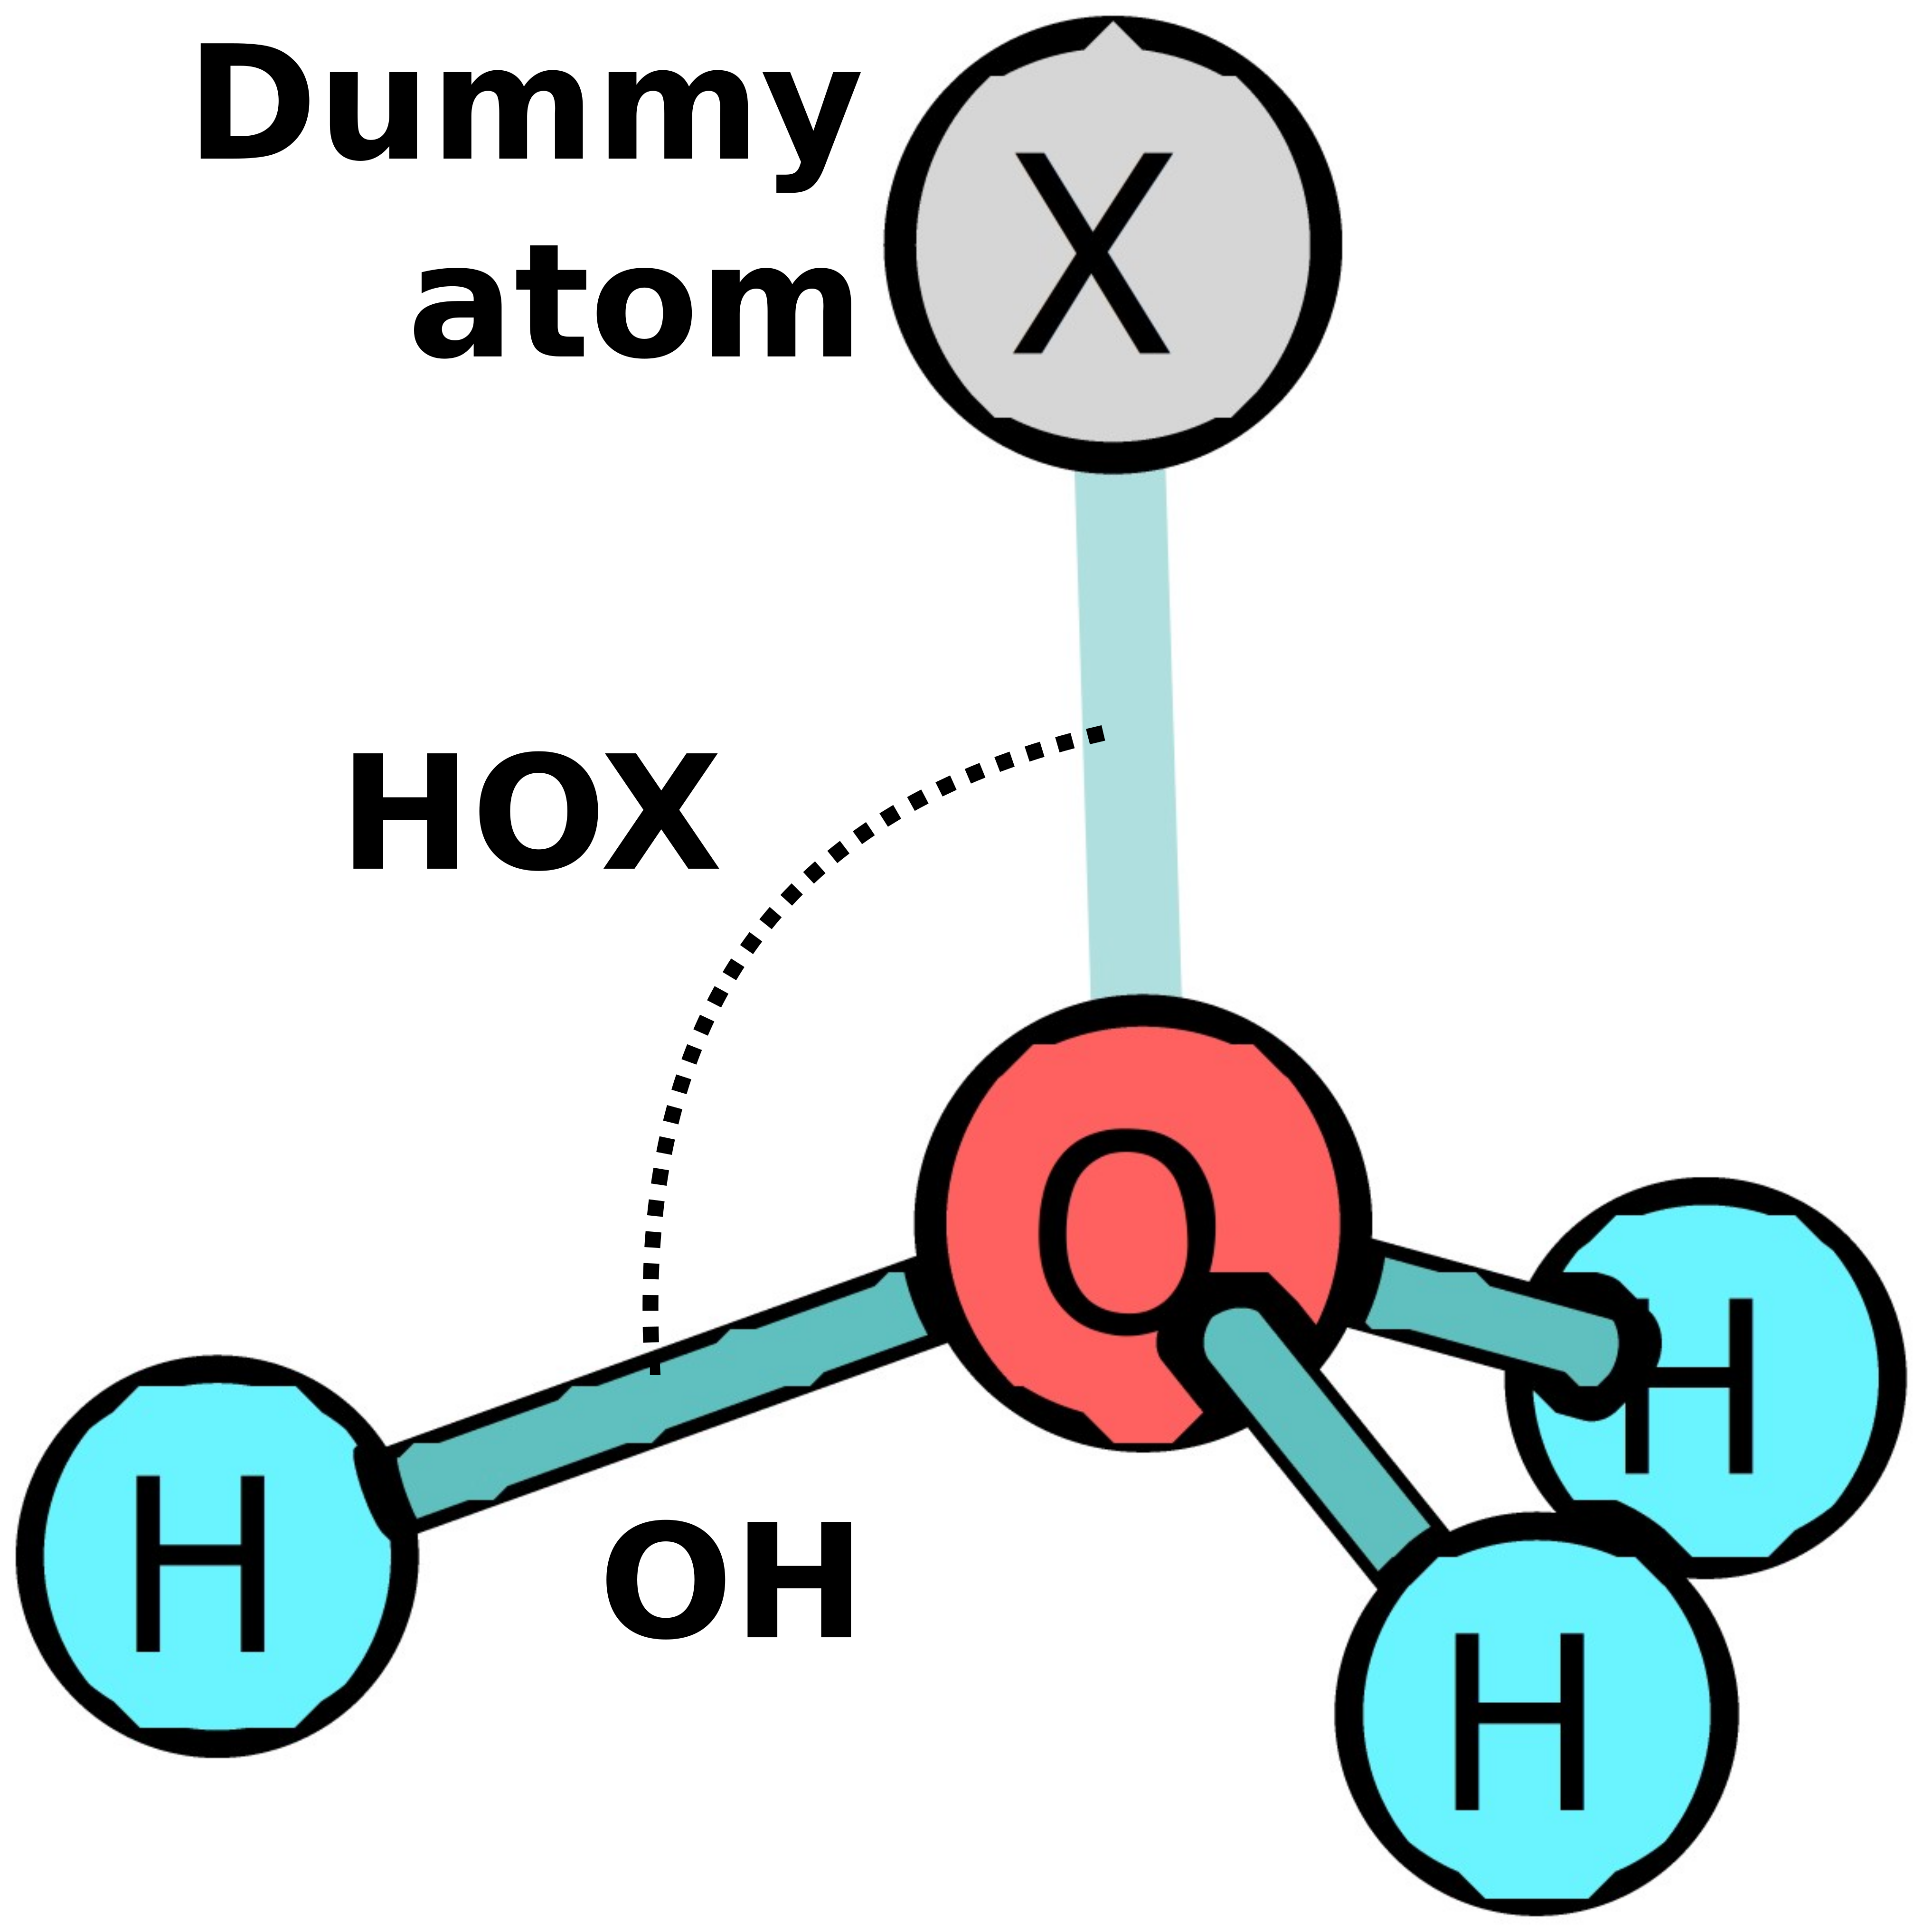
\includegraphics[width=0.75\textwidth]{pics/zmat.png}
    \caption{Definition of hydronium ion internal coordinates. 
      The calculations perform a scan along the \ch{X-O-H} coordinates for all three hydrogens from \qtyrange{135}{90}{\degree}. 
      The \ang{120} dihedral angle indicates the relative position of hydrogen atoms.}
    \label{fig:internal_coords}
  \end{marginfigure}

  \item Localize the lowest-energy and transition structure along the PES and calculate the reaction barrier of the internal flip of the hydronium ion. 
  Whereas the energy of the pyramidal ion is comparable with the minimum on the PES, the energy of the optimized planar cation and the local maximum on the PES is different. 
  Why? Compare the geometries. 

  \item In the final step, rerun the calculations using the \texttt{MP2} method and compare your results. 
  You'll need to rerun the geometry optimization (for the pyramidal molecule) using the MP2 level of theory so you get the right bond length to run the PES scan of the umbrella mode. 
  Try plotting both PES scan curves in one plot to compare methods. 
  Look at the difference in final energies and the difference in the barrier energy for the two methods. 


\end{itemize}

\section*{Lab report}

For the lab report, please prepare following data.\sidenote{This is the bare minimum; there are couple of open questions in the text that you should try to assess.}
All of this can be done in the Discussion section of the Jupyter notebook. 
When you are finished, export the finished document as a PDF file  by clicking \menu{File>Export Notebook As…>Export Notebook to PDF} and email that PDF to me. 

\begin{enumerate}
  \item Plot the Total Energy vs. number of basis functions for a hydrogen atom for all methods used in Problem 1. 

  \item Plot the binding curves for HF using Hartree-Fock and PBE1PBE methods. Find the minimum distance and compute the atomization energy. 
  Plot the dipole moment as a function of the bond distance. 
  Plot both methods in the same image. You can do this with the \Verb{plt.plot()} method from the Matplotlib library. 
  If you made the distances into the index for your dataframe, you can call those values with \Verb{df.index.values}. 
  Multiple sets of \emph{x-y} data can be plotted with \Verb{plt.plot(x1, y1, x2, y2)}, where \Verb{x1}, ... are the various lists of \emph{x} and \emph{y} data. 

  \item Prepare tables listing molecular vibrations in a hydronium ion in planar and pyramidal geometries. 
  Make sure the wavenumbers are shown for all molecular vibrations. 

  \item Plot the PES along the HOX coordinate using HF and MP2 methods. 
  Use \unit{\kcal\per\mol} for the \( y \)-axis. 
  Compute the heigh of the barrier separating two pyramidal structures (the energy required to pass over the planar intermediate on the PES). 
  
\end{enumerate}



\clearpage

\appendix
%!TEX root = ./Intro_to_CC.tex 

\subsection{Appendix I: Bash and vi}
\label{app:bash}

Bash is a Unix shell and command language for the GNU Project and the default shell on Linux and OS X systems. We will use it to execute most programs and exercises. Below you find a list of the most import commands. Items in quotes indicate user-selected input (a directory/file name, a string of text, etc.). Bash furthermore offers a full programming language (often implemented via shell scripts) to automate tasks, e.g., via loops.
\marginnote[-4\baselineskip]{
A note on \emph{relative} and \emph{absolute} paths: Say you were giving directions to a location. You have two methods you can describe getting to the location:
\begin{itemize}
  \item Relative to where you stand, or
  \item Relative to a landmark.
\end{itemize}
Both descriptions get you to the same location, but the former only works from your current location (``take a left, then a right, go through two lights then take another right'' wouldn't necessarily work from the next town over, but works from where you stand).

In file systems, if you have \Verb{/home/user/documents/data.txt}, that's an absolute path (the starting \Verb{/} indicates the root of the drive). If you have \Verb{documents/data.txt}, it will only work so long as you're starting from \Verb{/home/user}. If you start in \Verb{/home/user/documents} you would need a \Verb{../} to get there correctly using the relative path. 

However, no matter where you are on the hard drive, \Verb{/home/user/documents/data.txt} is a definitive way to get to that file.} 

\begin{itemize}
  \item \textbf{Basic navigation:}
  \begin{description}[
    font=\ttfamily\upshape,
    align=left,
    style=nextline,
    itemindent=*]
    \item[ls] list all files and folders 
    \item[ls "dir-name"] list files in the directory.
    \item[ls -lh] Detailed (\textbf{l}ong) list, \textbf{h}uman readable
    \item[ls -l mypics/*.jpg] list only the jpeg files in the ``mypics'' directory
    \item[cd "folderName"] change directory
    \item[cd ..] go up one folder, tip: string together multiple folders \Verb{../../..}
  \end{description}
  
  \item \textbf{Basic file operations:}
  \begin{description}[
    font=\ttfamily\upshape,
    align=left,
    style=nextline,
    itemindent=*]
    \item[cat "file"] show all contents of a file
    \item[head "file"] show the top 10 lines of a file
    \item[tail -n5 "file"] show the last 5 lines of a file

    \item[mkdir "dir-name"] creates a new directory entitled ``dir-name'' (called folder in Windows and macOS) 
    \item[cp "file1" "file2"] - copy ``file1'' to ``file2'' 
    \item[cp image.jpg mypics/] - copy the file ``image.jpg'' to the ``mypics'' directory 
    \item[cp *.txt stuff/] copy all of files ending with ``.txt'' to the directory ``stuff''

    \item[mv "file1" "file2"] move (rename) ``file1'' to ``file2''
    \item[mv "file1" "dir-name>/"] move ``file1'' to directory ``dir-name'' 
    \item[mv "folderName/" ..] move directory up one level

    \item[rm "file1"] delete ``file1'' 
    \item[rm -r "junk\_stuff"] delete directory ``junk\_stuff'' and all files contained in it
  \end{description}
  
  \item \textbf{Extract, sort and filter data:}
  \begin{description}[
    font=\ttfamily\upshape,
    align=left,
    style=nextline,
    itemindent=*]
    \item[grep "someText" "file1"] search for the text ``someText'' in ``file1''.\sidenote{If your input has spaces, enclosing the input in double quotes (\Verb{"}) will preserve the spaces, e.g.,\Verb{"}Some quoted text\Verb{"}.} The \Verb{-i} flag tells grep to \textbf{i}gnore letter case (upper/lower).
    \item[grep -r "text" "folderName/"] return a list of lines in files contained in ``folderName'' with occurrences of ``text''
  \end{description}
  
  \item \textbf{Flow redirection and chain commands -- redirecting results of commands:}
  \begin{description}[
    font=\ttfamily\upshape,
    align=left,
    style=nextline,
    itemindent=*]
    \item[>] at the end of a command to redirect the result to a file (overwrites the contents of the file)
    \item[>>] at the end of a command to \textbf{append} the result to the end of a file
    \item[|] at the end of a command to send the output to another command 
    \item[\&] run the command in the background 
  \end{description}
  
  \item \textbf{Basic control:}
  \begin{description}[
    font=\upshape,
    align=left,
    style=nextline,
    itemindent=*]
    \item[\keys{\tab}] auto completion of file or command
    \item[\keys{\arrowkeyup}/\keys{\arrowkeydown}] See previous/next commands
    \item[\keys{\ctrl+R}] reverse search history
    \item[\keys{\ctrl+L}] clear the terminal
    \item[\Verb{!!}] repeat last command 
  \end{description}
\end{itemize}

\textbf{vi} is a terminal-based file edit program. By typing \Verb{vi} you open the program and create a new file that can be save later. By typing \Verb{vi "fileName"}, you open ``fileName'' to edit it. If ``fileName'' doesn't exist, you will create the new file and edit it immediately with this program. 

The editor, despite its simplicity in appearance, is a very powerful terminal-based tool with numerous key-bindings. Therefore, be careful what you press. In order to start editing the file, you first need to press \keys{I} (`\textbf{i}nsert') and then you can start typing. In order to save the file, press the \keys{Esc} key to exit the editing mode, then type \Verb{:} (\keys{\shift+;}) to enter the command mode in the bottom of the editor and type \Verb{wq} (for `\textbf{w}rite \textbf{q}uit'). Confirm with \keys{\return}. If you want to quit without saving the file, type \Verb{q!} in command mode. 







\vfill

\nocite{*}
\printbibliography[category=cited]% default title for `article` class: "References"

\DeclareFieldFormat{labelnumberwidth}{\textbullet}
\printbibliography[%
  title={Further Reading},%
  resetnumbers,%
  omitnumbers,%
  notcategory=cited,%
  ]

\end{document}
